\section{Papers}
\subsection{Neme (2013) Phylogenetic patterns of emergence of new genes
support a model of frequent de novo evolution}

    Citation \cite{neme_phylogenetic_2013}

    Uses phylostratigraphy to analyze trends across metazoans. A very
    powerful paper that does some of the same analyses I have done in At,
    which makes it a very nice source of comparisons.

    ``Younger genes are shorter, both with respect to gene length, as well
    as to open reading frame length. They contain also fewer exons and have
    fewer recognizable domains. Average exon length, on the other hand,
    does not change much over time'' pp. 1

    ``Conclusions: We suggest that the overall trends of gene emergence are
    more compatible with a de novo evolution model for orphan genes than a
    general duplication-divergence model. Hence de novo evolution of genes
    appears to have occurred continuously throughout evolutionary time and
    should therefore be considered as a general mechanism for the emergence
    of new gene functions.'' pp. 1

    ``With respect to gene length, the de novo model would predict that
    younger genes should be shorter than older genes, since it is unlikely
    that complex protein sequences emerge de novo. Rather one would expect
    that they could increase in size over evolutionary time. In the
    duplication-divergence model one would not expect length-dependence
    over time, since long and short genes should be equally likely subject
    to duplication at any time level.'' pp. 2.
    
    I do not agree. Long genes, if duplicated, would be more likely to have
    some region retain homology. If an ancient gene is duplicated and one
    daughter subsequently enters a period of neutral selection, her
    homology to her cousins will gradually decrease making her appear (to
    the phylostratigrapher) increasingly young, a Merlin effect). Assuming
    uniform mutation rates, a shorter gene will tend to reverse age more
    quickly.

    I further disagree with his reason for thinking de novo genes will be
    short. Of course it is true that specific information is not likely to
    appear by chance, but this is irrelevant. The length of monoexonic de
    novo proteins is determined by the distance between the start and stop
    codon.  This distance is distributed as a geometric random variable
    with a rate constant equal to the probability that a given codon is a
    stop codon. For polyexonic, cryptic de novo genes, length is determined
    by length and number of exons. Long polyexonic genes require multiple
    fortuitous events, thus are statistically unlikely to be long. Either
    way, length has nothing to do with protein complexity.

\subsection{Toll-riera (2013) Emergence of novel domains in proteins}

    Citation \cite{toll-riera_emergence_2013}

    Proteins are gradually lengthened by addition of young domains.

    ``\ldots we have identified all human young protein domains that have
    emerged in approximately the past 550 million years. \ldots We have
    found 426 different annotated young domains, totalling 995 domain
    occurrences, which represent about 12.3\% of all human domains. We have
    observed that 61.3\% of them arose in newly formed genes, while the
    remaining 38.7\% are found combined with older domains, and have very
    likely emerged in the context of a previously existing protein. Young
    domains are preferentially located at the N-terminus of the protein
    \ldots Furthermore, young domains show significantly higher
    non-synonymous to synonymous substitution rates than older domains
    using human and mouse orthologous sequence comparisons. This is also
    true when we compare young and old domains located in the same protein,
    suggesting that recently arisen domains tend to evolve in a less
    constrained manner than older domains. Conclusions: We conclude that
    proteins tend to gain domains over time, becoming progressively longer.
    We show that many proteins are made of domains of different age, and
    that the fastest evolving parts correspond to the domains that have
    been acquired more recently.'' pp. 1

    Genes in Eukaryotes tend to grow by addition of novel domains at the 3'
    (N-terminus) end.

    Apparently the way proteins gain domains has been thorougly studied
    \cite{chothia_evolution_2003, vogel_structure_2004,
    ekman_multi-domain_2005, moore_arrangements_2008,
    buljan_evolution_2009, marsh_how_2010, moore_dynamics_2011,
    ekman_quantification_2007}.

\subsection{Abrusan (2013) Integration of New Genes into Cellular Networks,
    and Their Structural Maturation} 

    Citation \cite{abrusan_integration_2013}

    ``I show that $1)$ The number of regulatory, protein–protein, and
    genetic interactions increases continuously with gene age, although
    with very different rates. New regulatory interactions emerge rapidly
    within a few million years, while the number of protein–protein and
    genetic interactions increases slowly, with a rate of 2-2.25 $\times$
    $10^{-8}$/year and 4.8 $\times$ $10^{-8}$/year, respectively. $2)$ Gene
    essentiality evolves relatively quickly: the youngest essential genes
    appear in proto-genes $\sim$14 MY old. $3)$ In contrast to
    interactions, the secondary structure of proteins and their robustness
    to mutations indicate that new genes face a bottle- neck in their
    evolution: proto-genes are characterized by high b-strand content, high
    aggregation propensity, and low robustness against mutations, while
    conserved genes are characterized by lower strand content and higher
    stability, most likely due to the higher probability of gene loss among
    young genes and accumulation of neutral mutations.'' pp. 1

    Builds off the Carvunis results.

    Sets out to test two things: $1)$ integration of orphans into networks
    $2)$ the continuity ngORF-protogene-gene continuity predicted by
    Carvunis.

\subsection{Wissler (2013) Mechanisms and Dynamics of Orphan Gene Emergence
in Insect Genomes} 

    Citation \cite{wissler_mechanisms_2013}

    Calculated the number of orphans in each of 30 insect genomes. Found an
    expected ~500 orphan genes per genome (~4\%). Of these, 43 \% for
    Formicidae species and 61\% for Attini species had matches to non-genic
    sequence.

    \begin{figure}[h!] \centering
        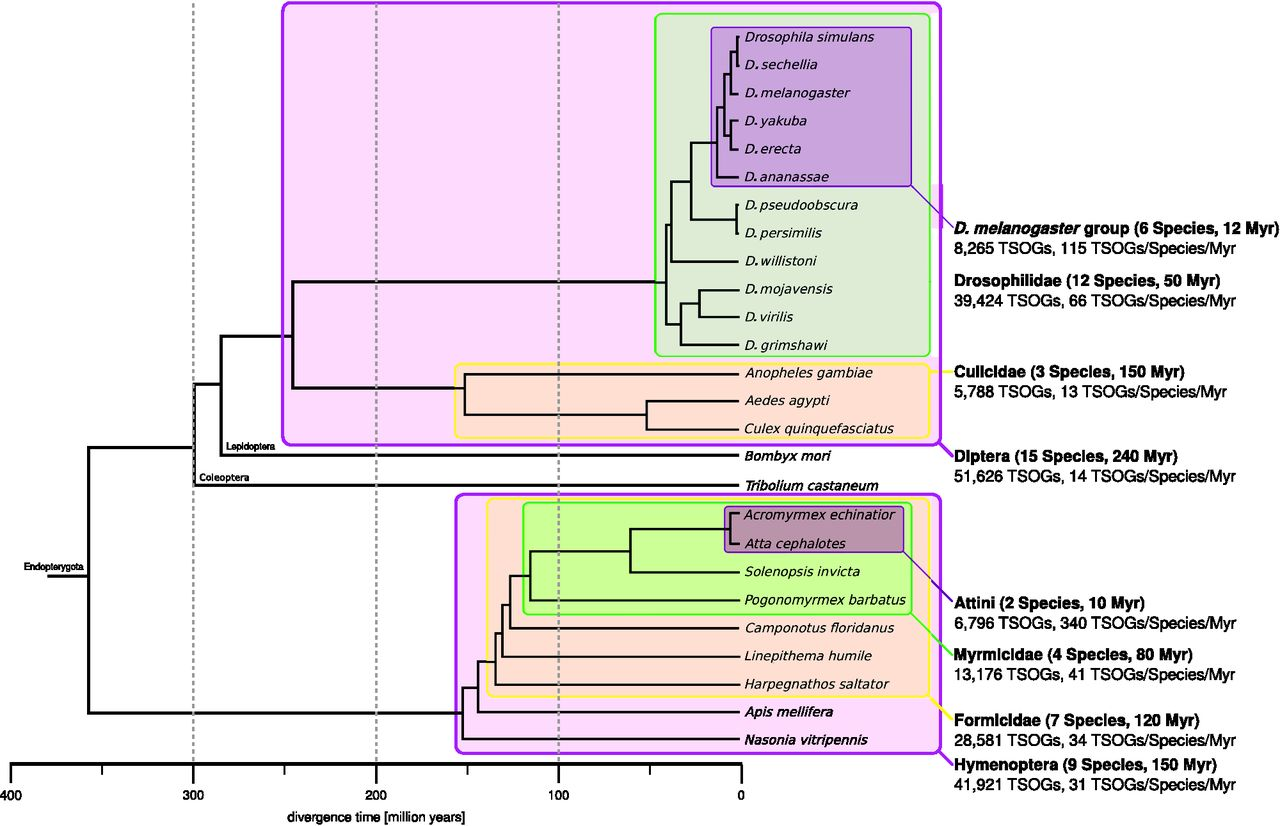
\includegraphics[scale=1]{wissler_insect_2013-fig2} \caption{
            Wissler \textit{et al.} Insect tree } \end{figure}

    \begin{figure}[h!] \centering
        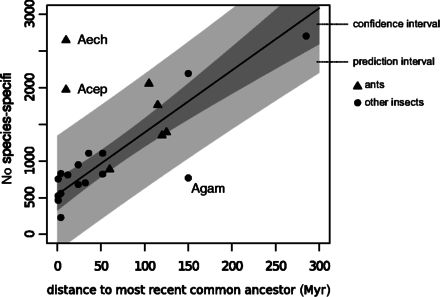
\includegraphics[scale=0.5]{wissler_insect_2013-fig1} \caption{
            Wissler \textit{et al.} orphan count versus separation from
        nearest relative } \end{figure}

    \begin{figure}[h!] \centering
        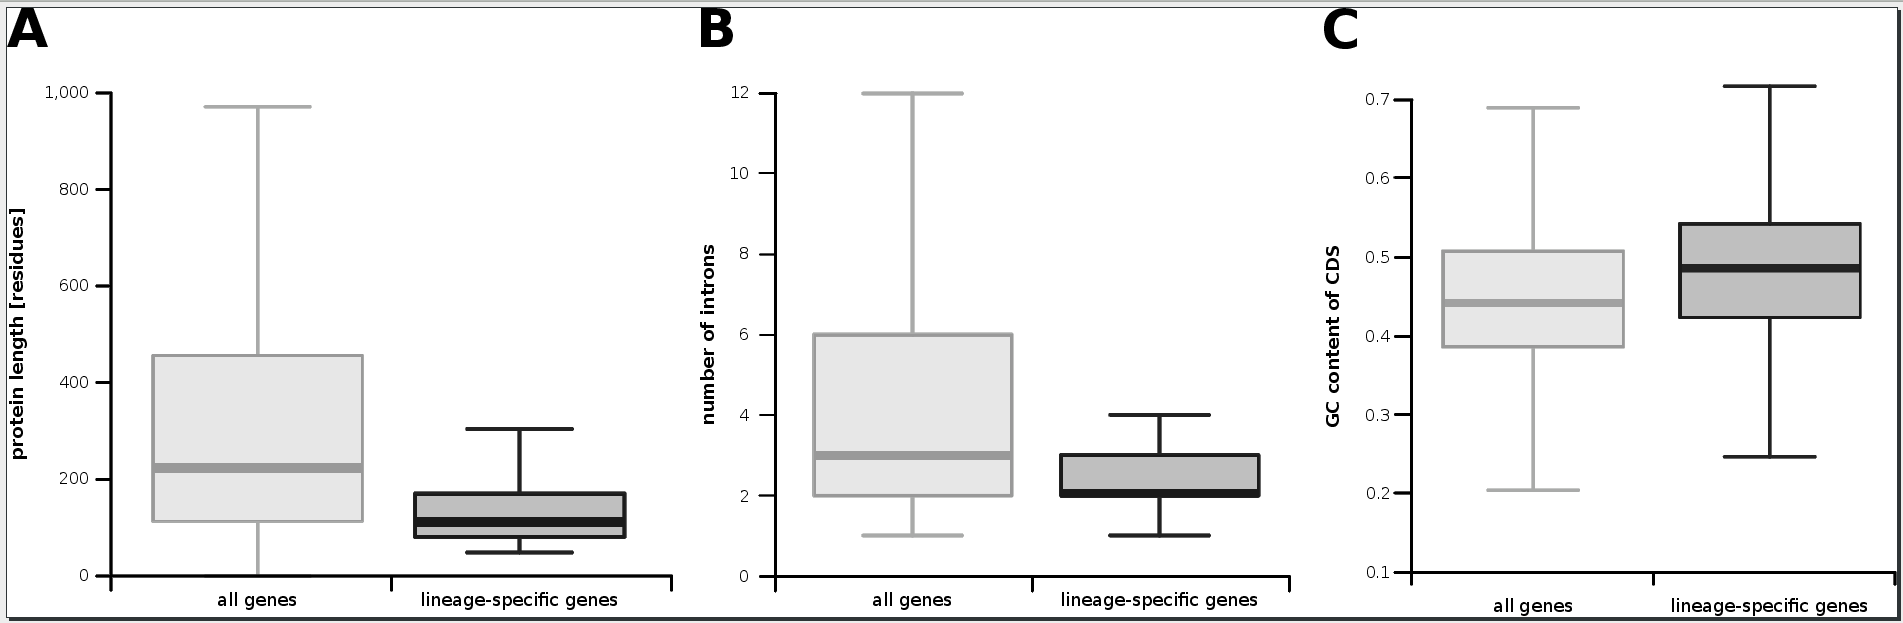
\includegraphics[scale=0.2]{wissler_insect_2013-supfig5} \caption{
            Wissler \textit{et al.} various traits } \end{figure}

    \FloatBarrier

\subsection{Thakur (2013) De Novo Transcriptome Sequencing and Analysis for
Venturia inaequalis, the Devastating Apple Scab Pathogen}

    Citation \cite{thakur_novo_2013}

    \begin{description}
        \item[Set A] 24571 unique genes with homology. 463 putative secreted
            proteins.
        \item[Set B] 32311 assembled transcripts without homology. 483 putative
            secreted proteins.
    \end{description}

    \begin{figure}[h!] \centering
        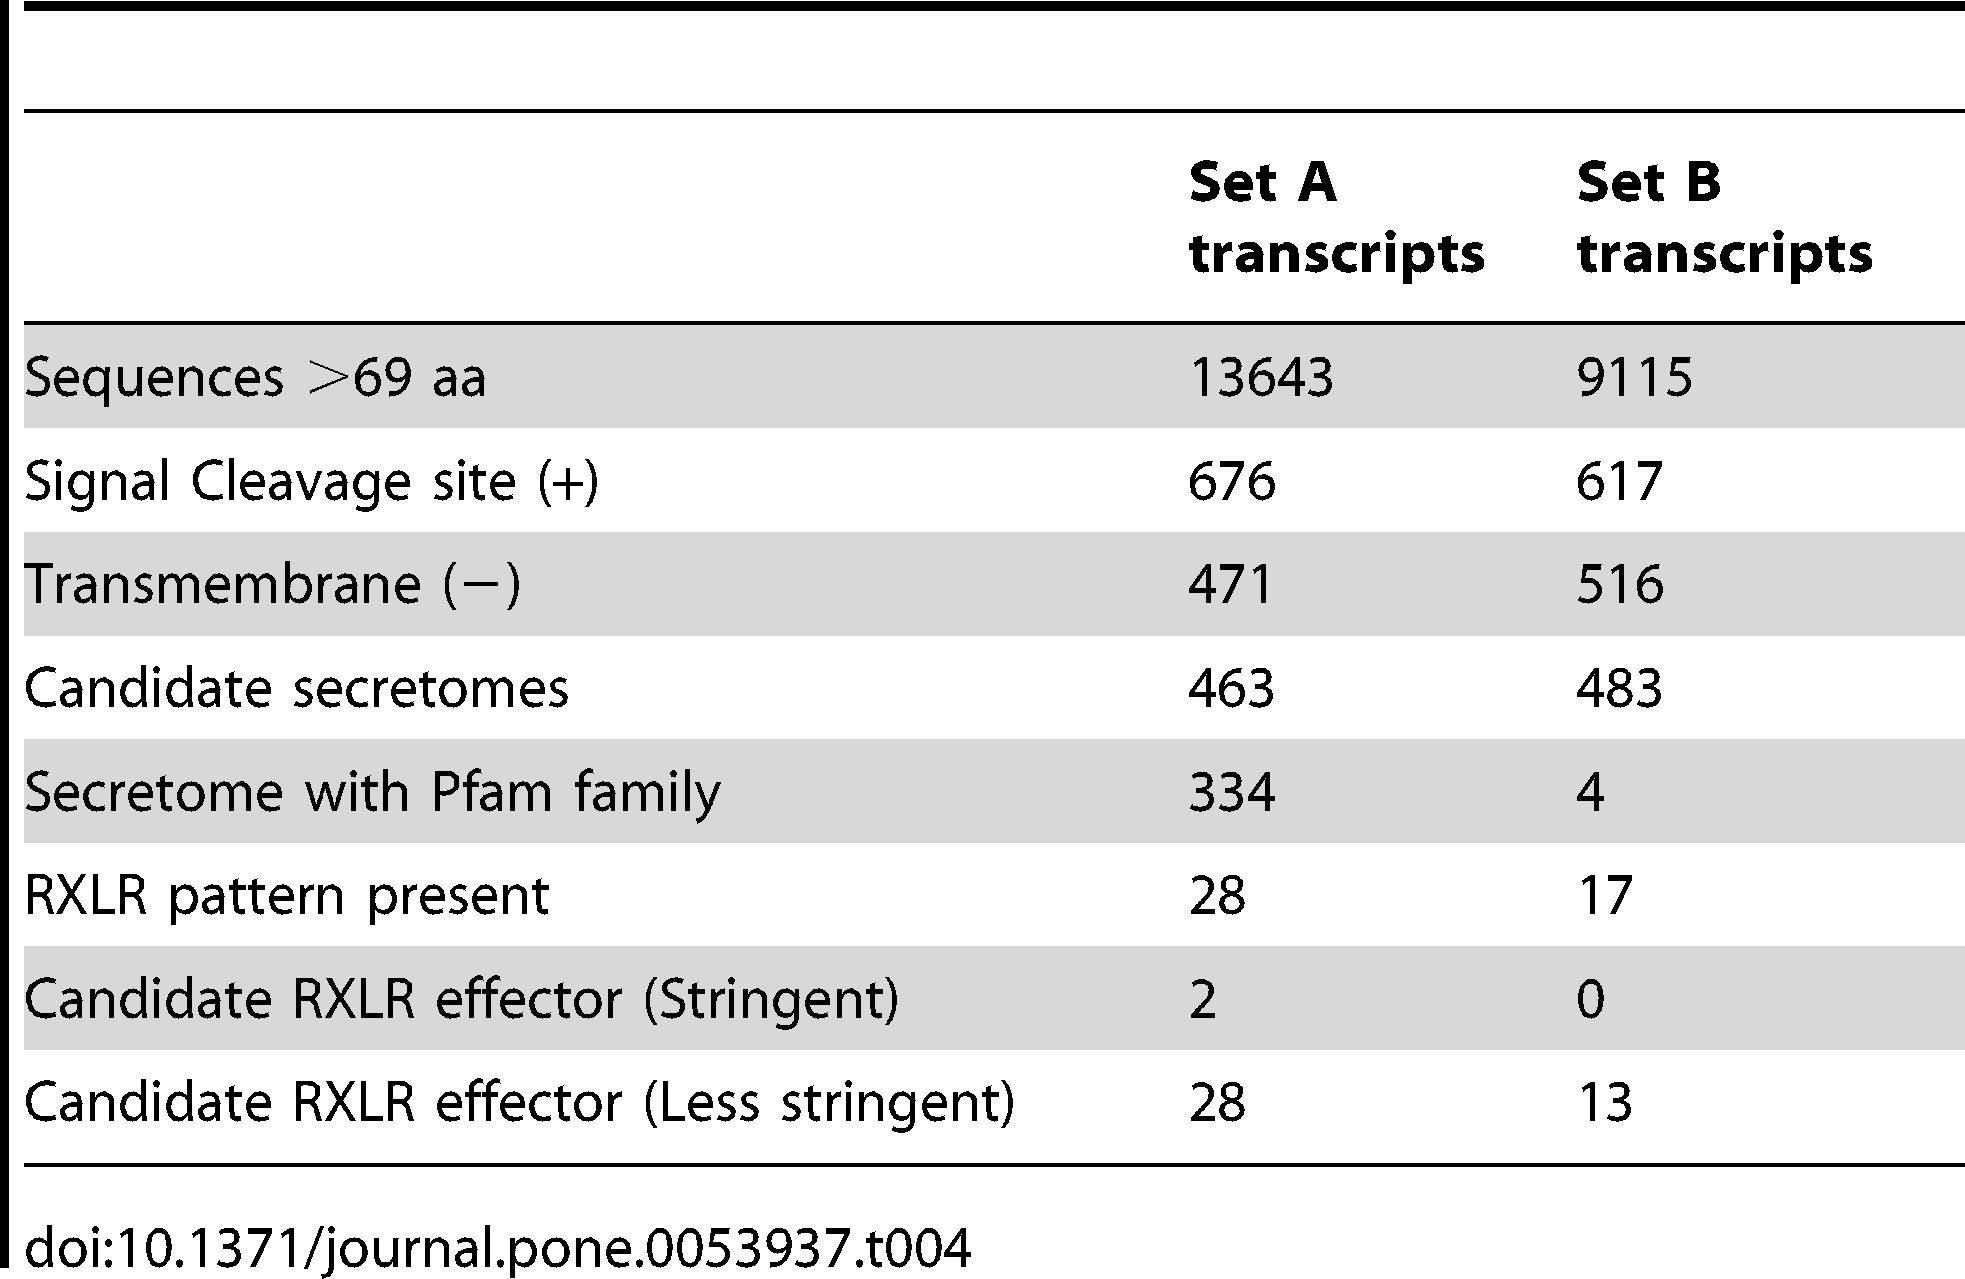
\includegraphics[scale=1]{thakur_denovo_2013-fig4}
        \caption{
            Thakur \textit{et al.} (fig 4) \textbf{Set A} has homology,
            \textbf{Set B} doesn't.
        }
    \end{figure}
    \FloatBarrier

\subsection{Gibson (2013) Why so many unknown genes? Partitioning orphans
from a representative transcriptome of the lone star tick Amblyomma
americanum}

    Citation \cite{gibson_why_2013}

    EST based estimate of orphan percentages in ticks.

    ``Expressed sequence tags (ESTs) were derived from different life stages
    and populations of A. americanum and combined with ESTs available from
    GenBank to produce 14,310 ESTs, over twice the number previously available.
    The vast majority (71\%) has no sequence homology to proteins archived in
    UniProtKB. We show that poor sequence or assembly quality is not a major
    contributor to this high representation by orphan genes. Moreover, most
    unannotated sequences are functional: a microarray experiment demonstrates
    that 59\% of functional ESTs are unannotated. Lastly, we attempt to further
    annotate our EST dataset using genomic datasets from other members of the
    Acari, including Ixodes scapularis, four other tick species and the mite
    Tetranychus urticae. We find low homology with these species, consistent
    with significant divergence within this subclass'' pp. 1

    ``We conclude that the abundance of orphan genes in A. americanum likely results
    from 1) taxonomic isolation stemming from divergence within the tick lineage
    and limited genomic resources for ticks and 2) lineage- specific genes needing
    functional genomic studies to evaluate their association with the unique
    biology of ticks.  The EST sequences described here will contribute
    substantially to the development of tick genomics. Moreover, the framework
    provided for the evaluation of orphan genes can guide analyses of future
    transcriptome sequencing projects.'' pp. 1

    Cites transcriptome projects from 12 mite species [hers, 24-35].

    71\% figure seems ridiculous, as the author is keenly aware. She discusses
    the problems. Many of the orphans may be due to issues with annotation,
    especially in the nearset neighbor. Tentative. More certainty requires a
    full transcriptome.

\subsection{Carvunis (2012) Proto-genes and de novo gene birth}

    Citation \cite{carvunis_proto-genes_2012}

    Introduces ngORF to proto-gene to mature gene model. Uses RNA-seq data
    as evidence of ORF transcription and ribosome footprinting as evidence
    of translation.

    proto-gene := transcribed AND translated ORF
    
    ``Such a reservoir of proto-genes would allow evolutionary innovations
    to be attempted without affecting existing genes'' pp. 1

    \begin{figure}[h!] \centering
        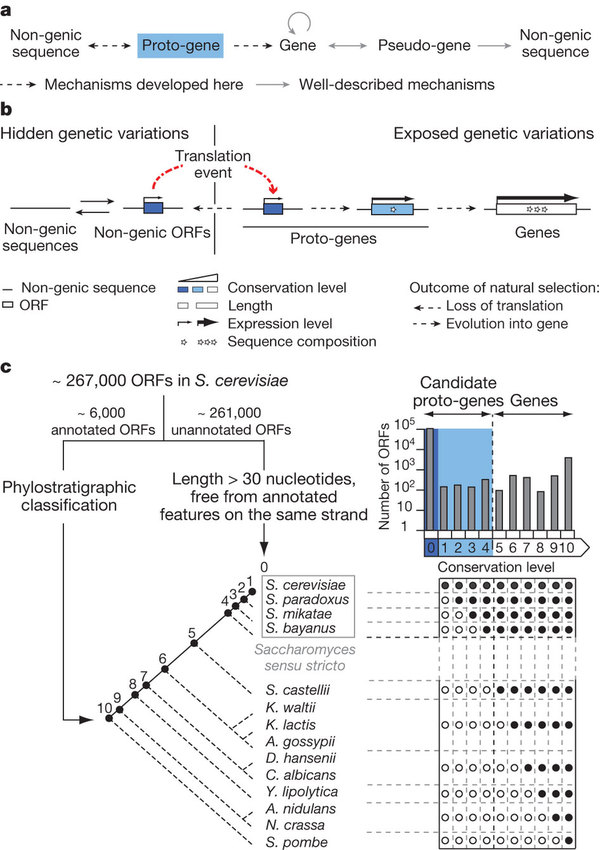
\includegraphics[scale=0.6]{carvunis_protogene-fig1} \caption{
            Carvunis (2012) protogenes and trees. Top right, number of ORFs
            assigned to each conservation level (logarithmic scale). A.
            gossypii, Ashbya (Eremothecium) gossypii; A. nidulans,
            Aspergillus nidulans; C. albicans (Saccharomycetales MRCA 490
            mya), Candida albicans; D. hansenii, Debaryomyces hansenii; K.
            lactis, Kluyveromyces lactis; K. waltii, Kluyveromyces
        (Lachancea) waltii; N. crassa, Neurospora crassa; S. pombe,
    Schizosaccharomyces pombe (Ascomycota MRCA ~800 mya).  } \end{figure}
    \begin{figure}[h!] \centering
        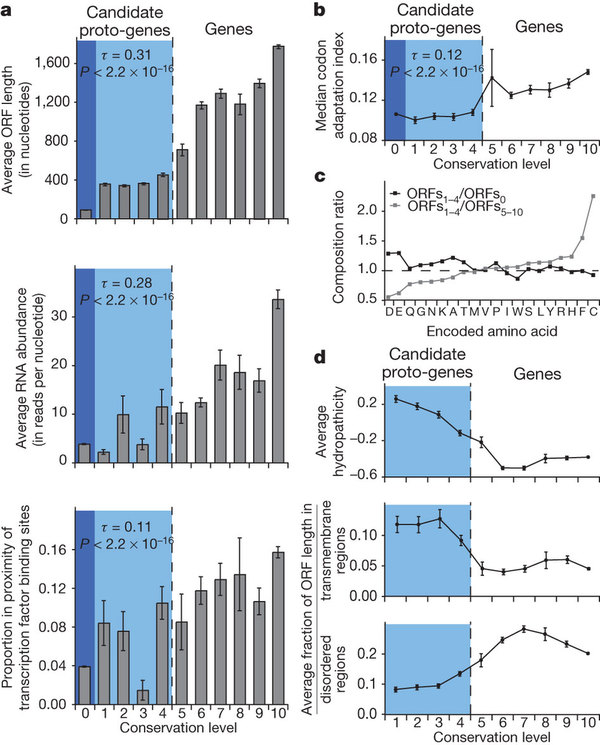
\includegraphics[scale=0.6]{carvunis_protogene-fig2} \caption{
            Carvunis (2012) trends in yeast
            \cite{carvunis_proto-genes_2012}.  ~14 million year spread
            between first 4 strata, ~800 million years from strata 10.  }
        \end{figure}
    \begin{figure}[h!] \centering
        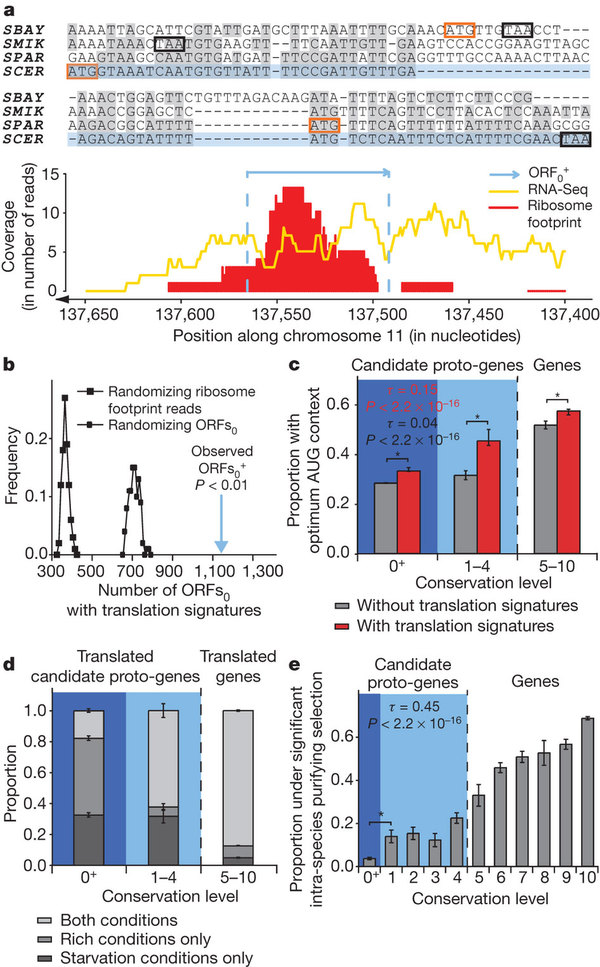
\includegraphics[scale=0.6]{carvunis_protogene-fig3} \caption{
        Carvunis (2012) ribosome binding, AUG optimal context, purifying
    selection, stress } \end{figure}
    \FloatBarrier

    Trends:

    \begin{enumerate}
        
        \item Increase in intrinsic disorder

        Disorder increases early, peals at a stratum ~490 mya, then falls.

        In At, the disorder jumps from low in ngORFs to high in orphans,
        remains steady, then falls significantly in the Viridiplantae and
        Eukaryota strata.

        \item Increase in codon optimization \item Increase in RNA abundance
    \item Increase in nearby transcription factor binding sites \item
    Increase in length \item Decrease in hydropathicity \end{enumerate}

    All of these, except transcription factors and hydropathicity, I have
    confirmed in \textit{A. thaliana}


\subsection{Colbourne (2011) The Ecoresponsive Genome of Daphnia pulex}

    Citation \cite{colbourne_ecoresponsive_2011}

    \begin{figure}[h!] \centering
        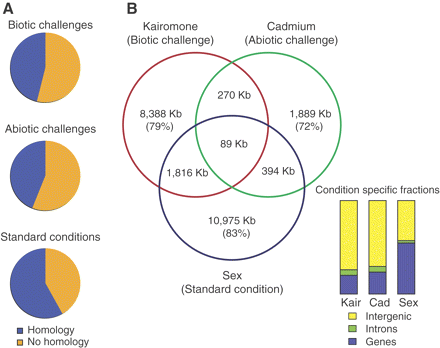
\includegraphics[scale=0.6]{colbourne_daphnia_2011-fig5} \caption{
            Colbourne (2011) fig5 Daphnia pulex
            \cite{colbourne_ecoresponsive_2011} } \end{figure}
        \FloatBarrier

\subsection{Moore (2011) The Dynamics and Evolutionary Potential of Domain
Loss and Emergence}

    Citation \cite{moore_dynamics_2011}


\subsection{Buljan (2010) Quantifying the mechanisms of domain gain in animal proteins}
    Citation \cite{buljan_quantifying_2010}

    In animals, proteins usually grow by fusion with the exons of adjacent
    genes or exonization of non-genic sequence.

    \textbf{``Background: Protein domains are protein regions that are shared
        among different proteins and are frequently functionally and
        structurally independent from the rest of the protein. Novel domain
        combinations have a major role in evolutionary innovation. However, the
        relative contributions of the different molecular mechanisms that
        underlie domain gains in animals are still unknown. By using animal
        gene phylogenies we were able to identify a set of high confidence
        domain gain events and by looking at their coding DNA investigate the
        causative mechanisms.}

    \textbf{``Results: Here we show that the major mechanism for gains of new
        domains in metazoan proteins is likely to be gene fusion through
        joining of exons from adjacent genes, possibly mediated by non-allelic
        homologous recombination.  Retroposition and insertion of exons into
        ancestral introns through intronic recombination are, in contrast to
        previous expectations, only minor contributors to domain gains and have
        accounted for less than 1\% and 10\% of high confidence domain gain
        events, respectively.  Additionally, exonization of previously
        non-coding regions appears to be an important mechanism for addition of
        disordered segments to proteins. We observe that gene duplication has
        preceded domain gain in at least 80\% of the gain events.}

    \textbf{``Conclusions: The interplay of gene duplication and domain gain
        demonstrates an important mechanism for fast neofunctionalization of
        genes.''}

    \begin{figure}[h!]
        \centering
        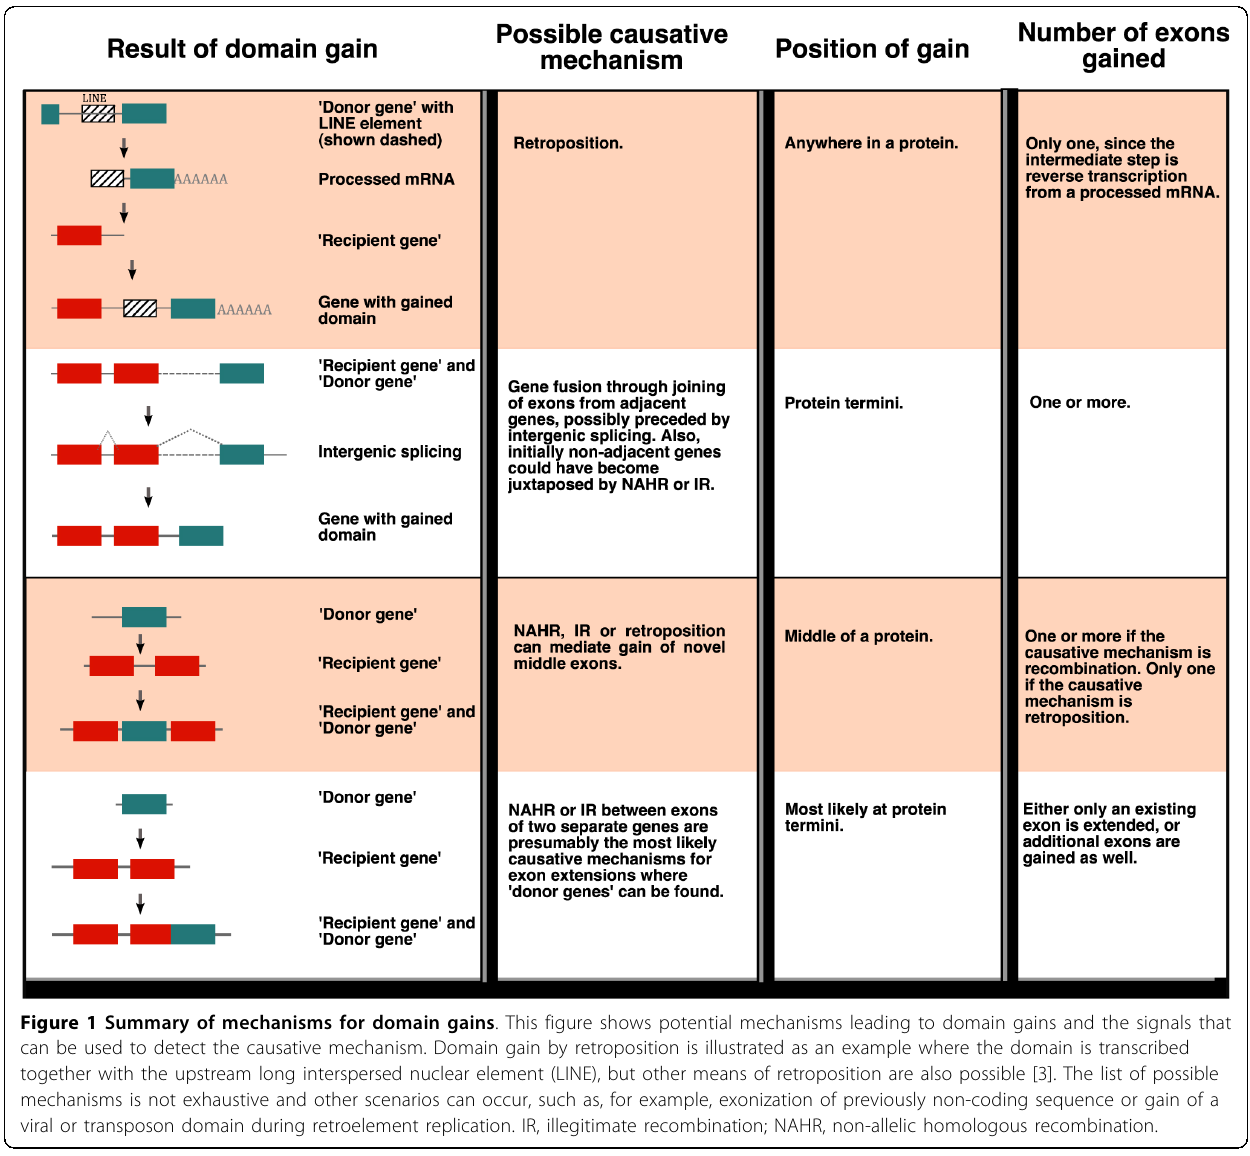
\includegraphics[height=0.7\textheight]{buljan-domain-2010-fig1}
        \caption{Buljan (2010)}
    \end{figure}

    \begin{figure}[h!]
        \centering
        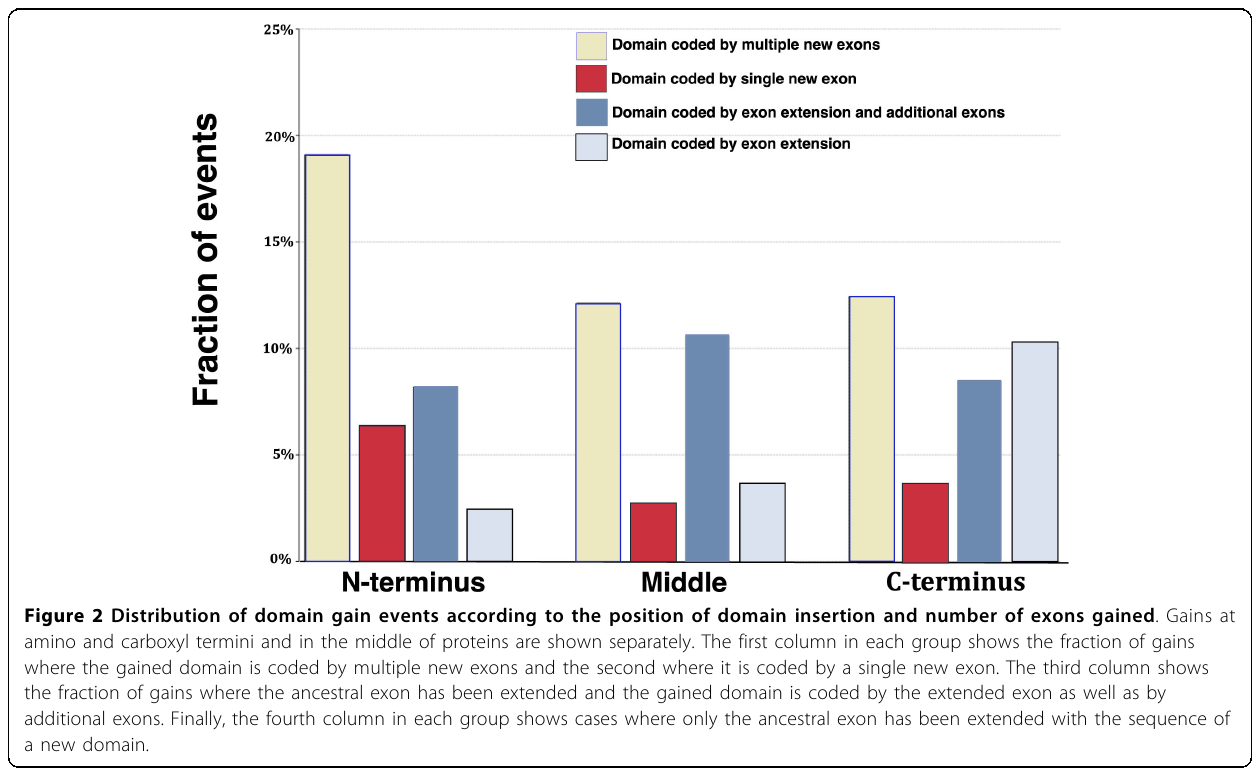
\includegraphics[width=0.9\textwidth]{buljan-domain-2010-fig2}
        \caption{Buljan (2010)}
    \end{figure}

    \begin{figure}[h!]
        \centering
        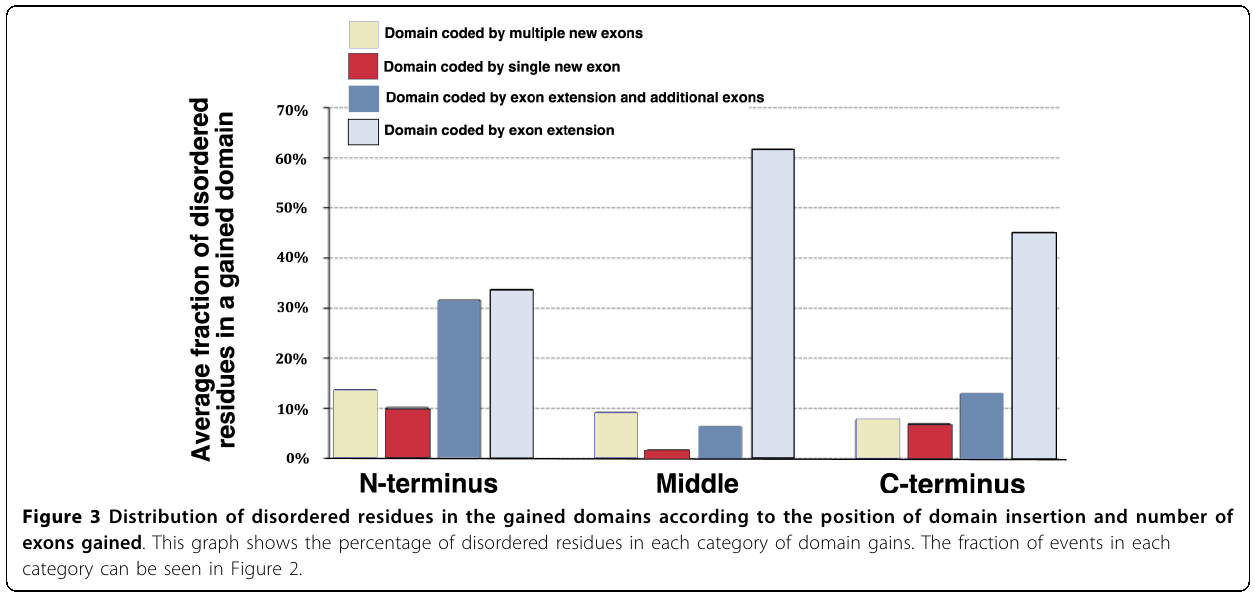
\includegraphics[width=0.9\textwidth]{buljan-domain-2010-fig3}
        \caption{Buljan (2010)}
    \end{figure}
    \FloatBarrier
    
\subsection{Gollery (2006) What makes species unique? The contribution of
proteins with obscure features}

    Citation \cite{gollery_what_2006}

\subsection{Ohno (1970) Evolution by gene duplication}

    Citation \cite{ohno_evolution_1970}

    Argues that new genes come almost exclusively from old genes. The idea
    is much older than this book, but Ohno is the oft cited champion of the
    idea.
